\documentclass[conference]{IEEEtran}
\IEEEoverridecommandlockouts

\usepackage[utf8]{inputenc}
\usepackage[T1]{fontenc}
\usepackage[spanish,es-noshorthands,es-tabla]{babel}
\usepackage{cite}
\usepackage{amsmath,amssymb}
\usepackage{graphicx}
\usepackage{booktabs}
\usepackage{float}
\usepackage{multirow}
\usepackage{tipa}
\usepackage{url}
\usepackage[hidelinks]{hyperref}
\usepackage{listings}
\lstset{basicstyle=\ttfamily\footnotesize, columns=fullflexible, keepspaces=true,
  frame=single, framerule=0.4pt, xleftmargin=4pt, xrightmargin=4pt, language=Python,
  commentstyle=\itshape, upquote=true}

% Símbolos fonéticos
\newcommand{\fz}{\textipa{z}}
\newcommand{\fdz}{\textipa{dz}}
\newcommand{\fZ}{\textipa{Z}}
\newcommand{\fdZ}{\textipa{dZ}}
\newcommand{\fs}{\textipa{s}}
\newcommand{\fts}{\textipa{ts}}
\newcommand{\fS}{\textipa{S}}
\newcommand{\ftS}{\textipa{tS}}
\newcommand{\dB}{\,dB}

\begin{document}

\title{Reducción del \textit{apitxat} en una voz sintética valenciana mediante ajuste fino multilocutor de Matcha-TTS con \textit{embeddings} de locutor mezclados y congelados}

\author{\IEEEauthorblockN{[Nombre y apellidos]}
\IEEEauthorblockA{Universitat Jaume I\\
Castelló de la Plana, España\\
pexposit@uji.es}}

\maketitle

\begin{abstract}
Las voces sintéticas en valenciano que se usan en aplicaciones de aprendizaje de la lengua deben ajustarse a la pronunciación normativa. La voz femenina \textit{Gina}, del modelo multilocutor Matxa (Matcha-TTS), presenta \textit{apitxat}: ensordece sistemáticamente las sibilantes sonoras /\fz/, /\fdz/, /\fZ/ y /\fdZ/, rasgo dialectal ajeno al estándar de la Acadèmia Valenciana de la Llengua (AVL). Este trabajo propone una métrica acústica de sonoridad basada en la caída de energía por debajo de 400~Hz en la zona de fricción y la emplea para guiar el ajuste fino de Matxa con unas 90\,000 grabaciones del \textit{Diccionari normatiu valencià} (DNV) más clips de Gina. Se comparan tres estrategias: eliminar los clips de Gina con sibilantes sonoras, inicializar su \textit{embedding} de locutor como una mezcla al 50\,\% con una locutora del DNV y, además, congelar ese \textit{embedding} durante el entrenamiento. El contraste sonora/sorda de Gina pasa de 1,4--3,1\dB{} a 16,5$\pm$1,1\dB{} con la tercera estrategia, dentro del rango de los locutores humanos del DNV (16,1--20,3\dB). Al mismo tiempo, la voz conserva una similitud de locutor de 0,930 respecto a la original, la calidad estimada (PESQ$\approx$4,06) y la inteligibilidad (WER 5,7\,\%). Los resultados indican que, en Matxa, la sonoridad de las sibilantes está codificada en gran parte en el \textit{embedding} de locutor, y que fijar ese \textit{embedding} permite que el decodificador recupere el timbre sin reintroducir el ensordecimiento.
\end{abstract}

\begin{IEEEkeywords}
síntesis de voz, Matcha-TTS, ajuste fino, \textit{embedding} de locutor, valenciano, sonoridad, sibilantes, \textit{apitxat}
\end{IEEEkeywords}

% ==========================================================================
\section{Introducción}
% ==========================================================================

Las aplicaciones de aprendizaje de lenguas utilizan cada vez más voces sintéticas para leer en voz alta palabras, frases y diálogos. En ese contexto la voz actúa como modelo de pronunciación: el alumnado la imita. Por ello no basta con que la voz sea natural e inteligible, sino que debe ajustarse a la norma que se enseña. Este trabajo surge del desarrollo de ParlaVal, una aplicación de aprendizaje del valenciano que incorpora un laboratorio de voz basado en el modelo catalán Matxa~\cite{matxa}, una versión multilocutor y multiacento de Matcha-TTS~\cite{mehta2024matcha} publicada por el Projecte Aina.

La voz femenina \textit{Gina} (locutora 7 de Matxa) se eligió por su timbre y su claridad, pero presenta \textit{apitxat}. El \emph{valenciano apitxat} es una variedad dialectal del valenciano, propia de la zona central, que se caracteriza por el ensordecimiento de determinadas consonantes sonoras~\cite{recasens1996}.

Este rasgo afecta sobre todo a las \emph{sibilantes}. Son sonidos consonánticos que se producen estrechando el canal vocal hasta generar un ruido de fricción. Pueden ser de dos tipos:
\begin{itemize}
\item \emph{sonoras}, si las cuerdas vocales vibran durante su articulación, como /\fz/ en \textit{casa};
\item \emph{sordas}, si las cuerdas vocales no vibran, como /\fs/ en \textit{costat}.
\end{itemize}

El \emph{ensordecimiento de sibilantes} es el fenómeno por el que ciertos fonemas sonoros se pronuncian como sus correspondientes sordos:
\begin{itemize}
\item /\fz/ $\rightarrow$ [\fs];
\item /\fdz/ $\rightarrow$ [\fts];
\item /\fZ/ $\rightarrow$ [\fS];
\item /\fdZ/ $\rightarrow$ [\ftS].
\end{itemize}

Por ejemplo, una hablante apitxada pronuncia:
\begin{itemize}
\item \textit{casa} se pronuncia [\textipa{"kasa}] en lugar de [\textipa{"kaza}];
\item \textit{dotze} se pronuncia [\textipa{"dotse}] en lugar de [\textipa{"dodze}];
\item \textit{platja} se pronuncia [\textipa{"platSa}] en lugar de [\textipa{"pladZa}].
\end{itemize}
La normativa de la AVL~\cite{gnv2006} y la pronunciación de referencia del \textit{Diccionari normatiu valencià} (DNV)~\cite{dnv} mantienen la oposición sonora/sorda, de modo que una voz apitxada no es adecuada como modelo.

El problema tiene dos dificultades. Por un lado, la oposición desaparece en la propia voz de la locutora, y no solo en la transcripción: aunque el fonemizador proporcione el símbolo /\fz/, Gina produce [\fs]. Por otro, las métricas habituales de un ajuste fino (pérdida del decodificador, WER, similitud de locutor) son casi insensibles a este rasgo, porque una /\fz/ ensordecida sigue siendo perfectamente inteligible.

Las contribuciones del trabajo son:
\begin{enumerate}
\item una métrica acústica simple y reproducible de la sonoridad de las sibilantes en voz sintética, con un conjunto de cinco oraciones (26 sibilantes) diseñado para detectar el \textit{apitxat};
\item la evidencia empírica de que, en Matxa, la sonoridad de las sibilantes está ligada al \textit{embedding} del locutor, obtenida interpolando \textit{embeddings} en inferencia;
\item una receta de ajuste fino, que combina filtrado de datos con un \textit{embedding} mezclado y congelado, que elimina el ensordecimiento sin perder el timbre ni la calidad; y
\item una evaluación objetiva con varias semillas que cuantifica el compromiso entre sonoridad y timbre a lo largo del entrenamiento.
\end{enumerate}

% ==========================================================================
\section{Trabajos relacionados}
% ==========================================================================

\subsection{Síntesis multilocutor con \textit{flow matching}}
Matcha-TTS~\cite{mehta2024matcha} es un modelo acústico \emph{no autorregresivo}. Para entender qué significa conviene compararlo con la alternativa:
\begin{itemize}
\item \emph{Modelo autorregresivo}, como Tacotron~2. Genera el espectrograma fotograma a fotograma, y cada fotograma depende de los que ya ha producido. Por ese encadenamiento no se puede paralelizar, así que es lento. Además, un error en un punto se arrastra a todo lo que sigue, y el modelo puede llegar a repetir o saltarse palabras o no saber cuándo parar.
\item \emph{Modelo no autorregresivo}, como Matcha-TTS. Decide de antemano cuánto dura cada fonema y, con ello, la longitud total del audio. Después genera todos los fotogramas a la vez, en paralelo, lo que lo hace más rápido y más estable.
\end{itemize}

Matcha-TTS tiene dos partes:
\begin{itemize}
\item un codificador de texto y un predictor de duraciones, que deciden cuántos fotogramas ocupa cada fonema y alinean así los fonemas con los fotogramas;
\item un decodificador entrenado con \textit{conditional flow matching}~\cite{lipman2023flow}, que transforma ruido gaussiano en un mel-espectrograma integrando una ecuación diferencial ordinaria (ODE) en pocos pasos.
\end{itemize}

Estos pasos de la ODE no avanzan en el tiempo del audio. Cada uno refina la frase entera a la vez, de modo que el decodificador sigue siendo no autorregresivo. Como el punto de partida es ruido aleatorio, la misma red produce realizaciones algo distintas según la semilla, lo que obliga a evaluar con varias semillas (Sección~\ref{sec:eval}).
El \emph{embedding del locutor} (\textit{speaker embedding}) es una representación matemática de las características de una voz, en forma de vector de números, que permite identificar o diferenciar hablantes. En la variante multilocutor, cada locutor tiene su propio \textit{embedding}, aprendido durante el entrenamiento, que condiciona tanto el codificador como el decodificador. Matxa~\cite{matxa} entrena esta arquitectura con varios locutores y acentos del catalán. El mel-espectrograma se convierte en onda con un vocoder neuronal, como alVoCat~\cite{alvocat}, basado en Vocos~\cite{siuzdak2023vocos}, o WaveNeXt~\cite{okamoto2023wavenext}.

\subsection{Identidad del locutor y pronunciación}
En la síntesis multilocutor se suele suponer que el \textit{embedding} codifica el timbre y que el contenido fonético procede del texto~\cite{jia2018transfer}. Sin embargo, el \textit{embedding} también absorbe rasgos sistemáticos del habla de cada locutor, como el acento, el ritmo o los procesos fonológicos regulares, porque son tan constantes como el timbre. Este trabajo aprovecha precisamente esa propiedad: si el ensordecimiento vive en el \textit{embedding}, se puede tratar actuando sobre él.

\subsection{Acústica de la sonoridad en fricativas}
Las \emph{fricativas sonoras} son consonantes que se producen haciendo pasar el aire por un estrechamiento, lo que causa fricción, mientras vibran las cuerdas vocales. Ejemplos son /\fz/ y /\fZ/. Acústicamente combinan ruido turbulento de alta frecuencia con la vibración de las cuerdas vocales. Esta vibración se observa como una ``barra de sonoridad'' de baja frecuencia, por debajo de unos 400--500~Hz, que se mantiene durante la fricción. En las fricativas sordas las cuerdas vocales no vibran, así que esa energía cae bruscamente~\cite{stevens1998,ladefoged1996}.

La \emph{F0} (frecuencia fundamental) es la frecuencia de vibración de las cuerdas vocales y está relacionada con la percepción del tono de la voz. Se utiliza, entre otras cosas, para distinguir voces masculinas y femeninas. En principio, la presencia de F0 delata la sonoridad. Sin embargo, los detectores de F0 como pYIN~\cite{mauch2014pyin} tienden a fallar en las sibilantes, que son segmentos cortos y con mucho ruido. Por eso este trabajo mide directamente la energía en baja frecuencia.

% ==========================================================================
\section{Sistema base y datos}
% ==========================================================================

\subsection{Modelo y fonemización}
Se parte del punto de control publicado de \texttt{matxa-tts-cat-multiaccent}, que funciona a 22,05~kHz, y del vocoder alVoCat. Matxa recibe fonemas en lugar de letras, así que antes de sintetizar hay que convertir el texto en una transcripción fonética. Para ello se comparan dos fuentes:
\begin{itemize}
\item \emph{eSpeak} (eSpeak NG~\cite{espeakng}), un sistema de síntesis de voz de código abierto. Aquí se usa su módulo de conversión de texto a fonemas para generar las pronunciaciones, y es la fonemización por defecto de Matxa.
\item \emph{AVL}, las transcripciones fonéticas de la Acadèmia Valenciana de la Llengua, que se usan como referencia de la pronunciación normativa.
\end{itemize}
Para disponer de las transcripciones AVL se construyó un léxico a partir de 87\,760 entradas descargadas del DNV, que suman 96\,565 formas con su transcripción fonética. eSpeak discrepa del DNV en el 35\,\% de esas formas, principalmente en estos contrastes:
\begin{itemize}
\item hiato frente a diptongo, como en \textit{estació};
\item /e/ frente a /a/ átonas;
\item {[b]} frente a [\textipa{B}];
\item las aperturas vocálicas.
\end{itemize}
El fonemizador ``AVL'' usa el léxico cuando la palabra está en él y eSpeak en el resto de casos, conservando el \textit{sandhi} de eSpeak. El \emph{sandhi} es el fenómeno fonético por el que los sonidos se modifican por influencia de los sonidos vecinos, especialmente en el contacto entre palabras. Puede provocar sonorizaciones legítimas: en \textit{roses al jardí}, la \textit{-s} final de \textit{roses} se pronuncia [\fz] porque la sigue una vocal.

\subsection{Corpus de ajuste fino}
La Tabla~\ref{tab:datos} resume las fuentes. Las grabaciones del DNV aportan dos voces humanas, una femenina y una masculina, que pronuncian palabras aisladas según la norma. Se separaron por F0, porque la voz masculina ronda los 90~Hz y la femenina los 190~Hz, y se etiquetaron con la transcripción AVL del propio diccionario. Los clips de Gina son sintéticos y proceden de un ajuste fino previo con palabras cortas. Se etiquetan con eSpeak porque eso es lo que la voz pronuncia realmente: si se etiquetaran con AVL, el modelo aprendería que el símbolo /e/ suena [a]. Para que Gina no quede diluida entre las grabaciones del DNV, sus clips se repiten 10 veces.

\begin{table}[t]
\centering
\caption{Corpus de entrenamiento (partición de entrenamiento)}
\label{tab:datos}
\begin{tabular}{@{}llrr@{}}
\toprule
Locutor (id) & Etiquetas & Clips & Tras filtrar \\
\midrule
DNV, mujer (5) & AVL & 41\,883 & 41\,883 \\
DNV, hombre (4) & AVL & 47\,913 & 47\,913 \\
Gina (7), $\times$10 & eSpeak & 2\,038 & 1\,468 \\
\midrule
Total de líneas & & 110\,136 & 104\,436 \\
\bottomrule
\end{tabular}
\vspace{2pt}

{\footnotesize Las grabaciones del DNV suman 25,8~h. ``Tras filtrar'': sin los clips de Gina cuya transcripción contiene /\fz/ o /\fZ/ (v2--v4).}
\end{table}

El primer modelo ajustado con este corpus, \textbf{avl-v1}, adoptó correctamente la pronunciación AVL en vocales, hiatos y oclusivas, y conservó el timbre de Gina. Sin embargo, \emph{siguió siendo apitxat} (Sección~\ref{sec:diag}).

% ==========================================================================
\section{Medida del \textit{apitxat}}\label{sec:diag}
% ==========================================================================

\subsection{Oraciones de prueba}
Se diseñaron cinco oraciones que contienen 26 sibilantes objetivo: 16 sonoras y 10 sordas de control. Las sibilantes finales en contacto con vocal o consonante sonora se excluyeron, porque el \textit{sandhi} las sonoriza de forma legítima.
\begin{enumerate}
\item \textit{Ma casa és bonica i mon cosí viu al costat de l'església.}
\item \textit{Tinc dotze roses al jardí i onze rosses al pati.}
\item \textit{El jove menja formatge a la platja al migdia.}
\item \textit{El xiquet deixa el cotxe davant de la caixa.}
\item \textit{Les zones de la presó són grises i la sessió és seriosa.}
\end{enumerate}
Las sonoras se agrupan en tres clases: /\fz/ (9 casos), /\fdz/ (2) y /\fZ/,/\fdZ/ (5). La oración 4 solo contiene sordas palatales, y en las demás aparecen pares mínimos o casi mínimos, como \textit{roses}/\textit{rosses} o \textit{presó}/\textit{sessió}.

\subsection{Métrica de caída en baja frecuencia}
Para localizar cada fonema se usa un reconocedor fonético con \emph{alineamiento forzado} (\textit{forced alignment}). Este procedimiento sitúa en el tiempo los fonemas de un audio a partir de una transcripción de referencia: como ya se sabe qué fonemas contiene, solo hay que decidir dónde empieza y acaba cada uno. El reconocedor no sirve, en cambio, para juzgar la sonoridad: etiqueta [\fz] en el 99\,\% de los casos aunque no haya vibración. Por eso solo se aprovechan sus marcas temporales.

El análisis se apoya en dos herramientas:
\begin{itemize}
\item La \emph{STFT} (\textit{Short-Time Fourier Transform}, transformada de Fourier de tiempo corto). Divide la señal en tramos breves y calcula el contenido frecuencial de cada uno, lo que muestra cómo cambia ese contenido a lo largo del tiempo.
\item El \emph{espectrograma}, que es el resultado de la STFT: una representación, habitualmente visual, de cómo se distribuye la energía de las frecuencias de un audio a lo largo del tiempo.
\end{itemize}

Dado el intervalo alineado $[t_0,t_1]$ de una sibilante, se calcula el espectrograma de potencia $S(f,t)$. Este da la energía en cada frecuencia $f$ y cada instante $t$. Se obtiene con una STFT de 1024 puntos y saltos de 5~ms, sobre la ventana $[t_0-0{,}1,\ t_1+0{,}1]$~s, que incluye las vocales vecinas. A partir de él se suman tres energías por bandas de frecuencia:
\begin{align}
H(t) &= \textstyle\sum_{2{,}5\,\mathrm{kHz}<f<9\,\mathrm{kHz}} S(f,t), \\
M(t) &= \textstyle\sum_{0{,}4\,\mathrm{kHz}<f<2{,}5\,\mathrm{kHz}} S(f,t), \\
L(t) &= \textstyle\sum_{60\,\mathrm{Hz}<f<400\,\mathrm{Hz}} S(f,t).
\end{align}
Cada banda cumple una función:
\begin{itemize}
\item $H(t)$, \emph{energía de alta frecuencia} (2,5--9~kHz): es donde se concentra el ruido de fricción, y se usa para localizar la sibilante.
\item $M(t)$, \emph{energía de frecuencia media} (400~Hz--2,5~kHz): contiene la mayor parte de los formantes de las vocales, y se usa para distinguir la fricción de la vocal.
\item $L(t)$, \emph{energía de baja frecuencia} (60--400~Hz): recoge la vibración de las cuerdas vocales, y se usa para analizar si hay sonoridad.
\end{itemize}
La zona de fricción $\mathcal{F}$ se determina en tres pasos:
\begin{enumerate}
\item se toma el máximo de $H$ ponderado por una gaussiana de 60~ms centrada en el intervalo alineado;
\item se extiende mientras $H$ supere el 30\,\% de ese máximo;
\item se conservan solo los fotogramas en que $H(t)>0{,}5\,M(t)$, es decir, donde el ruido domina sobre los formantes.
\end{enumerate}
La \emph{métrica de caída en baja frecuencia} $C$, expresada en decibelios, compara la energía mediana de baja frecuencia durante la fricción con la máxima energía de baja frecuencia de toda la ventana. La \emph{caída} de la sibilante es
\begin{equation}
C = 10\log_{10}\frac{\operatorname{mediana}_{t\in\mathcal{F}} L(t)}{\max_t L(t)}\ \ [\mathrm{dB}],
\end{equation}
donde:
\begin{itemize}
\item $C$ es la caída de la sibilante, en decibelios (dB). Cuanto más negativa, más energía se pierde en la fricción respecto a la vocal y, por tanto, menos sonora es la sibilante.
\item $L(t)$ es la energía de baja frecuencia (60--400~Hz) en el instante $t$, que refleja la vibración de las cuerdas vocales.
\item $\mathcal{F}$ es la zona de fricción de la sibilante, es decir, el conjunto de fotogramas obtenido en los tres pasos anteriores.
\item $\operatorname{mediana}_{t\in\mathcal{F}} L(t)$ es el valor central de $L(t)$ en los fotogramas de la fricción. Se usa la mediana en lugar de la media para que unos pocos fotogramas de transición con la vocal no distorsionen el resultado.
\item $\max_t L(t)$ es la máxima energía de baja frecuencia de toda la ventana analizada. Corresponde a las vocales vecinas, que siempre son sonoras, y sirve de referencia para que la medida no dependa del volumen de la grabación.
\item $10\log_{10}(\cdot)$ convierte el cociente de energías en decibelios. Un cociente de 1 da 0~dB, es decir, la misma energía que la vocal. Un cociente de 0,01 da $-20$~dB, es decir, cien veces menos energía.
\end{itemize}
Una sibilante sonora conserva la barra de sonoridad y presenta caídas de unos $-5$ a $-20$\dB. Una sorda la pierde, con caídas de $-25$ a $-40$\dB. El \emph{contraste} de una voz es
\begin{equation}
\Delta = \overline{C}_{\text{sonoras}} - \overline{C}_{\text{sordas}},
\end{equation}
donde $\overline{C}_{\text{sonoras}}$ y $\overline{C}_{\text{sordas}}$ son las caídas medias de las sibilantes sonoras y sordas de las oraciones de prueba. Si una voz distingue bien unas de otras, $\Delta$ es grande. En una voz completamente apitxada, en cambio, vale cerca de 0\dB, porque pronuncia todas las sibilantes como sordas.

\subsection{Diagnóstico}
La Tabla~\ref{tab:base} muestra el contraste de los sistemas de partida. Los dos locutores del DNV alcanzan 16--20\dB. Todas las variantes de Gina se quedan en 1,4--3,1\dB, sea cual sea el fonemizador, el vocoder o la versión desplegada en el servidor, y también tras el ajuste avl-v1. El problema no está en la transcripción: el modelo recibe /\fz/ y produce [\fs].

\begin{table}[H]
\centering
\caption{Contraste sonora/sorda de los sistemas de partida}
\label{tab:base}
\begin{tabular}{@{}lrrr@{}}
\toprule
Sistema & $\overline{C}_{\text{son}}$ & $\overline{C}_{\text{sor}}$ & $\Delta$ (dB) \\
\midrule
DNV, mujer (grabación) & $-16{,}6$ & $-32{,}7$ & 16,1 \\
DNV, hombre (grabación) & $-12{,}9$ & $-33{,}2$ & 20,3 \\
\midrule
Gina, Matxa base, eSpeak & $-29{,}4$ & $-30{,}7$ & 1,4 \\
Gina, Matxa base, AVL & $-29{,}1$ & $-31{,}4$ & 2,2 \\
Gina, servidor de producción & $-30{,}0$ & $-32{,}7$ & 2,7 \\
Gina AVL, servidor (WaveNeXt) & $-34{,}3$ & $-37{,}4$ & 3,1 \\
avl-v1, época 29 & $-33{,}2$ & $-36{,}3$ & 3,1 \\
\bottomrule
\end{tabular}
\end{table}

\subsection{La sonoridad vive en el \textit{embedding}}
Para comprobar dónde reside el rasgo se interpoló, en inferencia y sobre avl-v1, el \textit{embedding} de Gina ($\mathbf{e}_7$) con el de la locutora femenina del DNV ($\mathbf{e}_5$):
\begin{equation}
\mathbf{e}_7(\alpha) = (1-\alpha)\,\mathbf{e}_7 + \alpha\,\mathbf{e}_5 .
\end{equation}
La Fig.~\ref{fig:mezcla} muestra el resultado. Por debajo de $\alpha=0{,}35$ el contraste no cambia. A partir de $\alpha\approx0{,}5$ crece de forma abrupta, hasta 17\dB{} con $\alpha=0{,}8$. Sin embargo, la similitud de locutor con Gina (Sección~\ref{sec:eval}) cae de 0,95 a 0,55. Por tanto, el modelo ya sabe producir sibilantes sonoras: lo que las ensordece es la región del espacio de \textit{embeddings} que ocupa Gina. La mezcla en inferencia por sí sola no basta, porque intercambia sonoridad por identidad.

\begin{figure}[t]
\centering
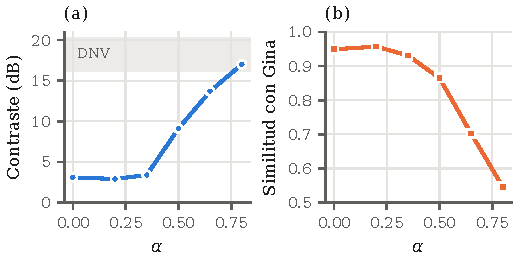
\includegraphics[width=\columnwidth]{figuras/fig_mezcla.pdf}
\caption{Interpolación del \textit{embedding} de Gina hacia la locutora del DNV en inferencia (avl-v1, época 29). (a) Contraste sonora/sorda; la franja gris es el rango de los locutores del DNV. (b) Similitud ECAPA con la voz original de Gina.}
\label{fig:mezcla}
\end{figure}

% ==========================================================================
\section{Estrategias de ajuste fino}
% ==========================================================================

Las tres estrategias parten del mismo punto de control de Matxa y del corpus de la Tabla~\ref{tab:datos}. Cada una añade un elemento a la anterior.

\textbf{v2: filtrado de datos.} Se eliminan los 570 clips de Gina (28\,\%) cuya transcripción contiene /\fz/ o /\fZ/, incluidas /\fdz/, /\fdZ/ y las sonorizaciones por asimilación. Esos clips enseñan al modelo que las sonoras de Gina son sordas. Sin ellos, toda la evidencia sobre cómo suenan las sibilantes sonoras procede de los locutores del DNV.

\textbf{v3: \textit{embedding} mezclado.} Además del filtrado, antes de entrenar se inicializa $\mathbf{e}_7 \leftarrow 0{,}5\,\mathbf{e}_7 + 0{,}5\,\mathbf{e}_5$. Así Gina arranca desde la región sonora del espacio de \textit{embeddings} (Fig.~\ref{fig:mezcla}a).

\textbf{v4: \textit{embedding} mezclado y congelado.} Igual que v3, pero la fila 7 de la matriz de \textit{embeddings} $\mathbf{E}$ no se actualiza. Se implementa con un \textit{hook} sobre el gradiente, que anula la fila en cada paso:
\begin{equation}
\frac{\partial \mathcal{L}}{\partial \mathbf{E}}\bigg|_{\text{fila }7} \leftarrow \mathbf{0}.
\end{equation}
En PyTorch basta con registrar una función que se ejecuta cada vez que se calcula el gradiente de la matriz y pone a cero la fila de Gina:
\begin{lstlisting}
filas = torch.tensor([7])        # Gina
emb = model.spk_emb.weight       # matriz E
emb.register_hook(
    lambda g: g.index_fill(0, filas.to(g.device), 0.0))
\end{lstlisting}
Para entender por qué la fila queda exactamente fija conviene recordar dos conceptos:
\begin{itemize}
\item \emph{Adam} es un algoritmo de optimización que actualiza los parámetros del modelo durante el entrenamiento a partir de los gradientes. Para ello lleva medias móviles (``momentos'') de los gradientes y de sus cuadrados.
\item El \emph{weight decay} es una técnica de regularización: penaliza los valores grandes de los pesos para limitar su crecimiento y ayudar a evitar el \emph{sobreajuste} (\textit{overfitting}). Hay sobreajuste cuando el modelo aprende demasiado los datos de entrenamiento y pierde capacidad de generalizar a datos nuevos.
\end{itemize}
Aquí se entrena sin \textit{weight decay}, es decir, sin aplicar esa penalización, que por sí sola desplazaría los pesos aunque su gradiente fuera nulo. Con Adam y sin \textit{weight decay}, un gradiente nulo desde el primer paso mantiene los momentos a cero, de modo que la actualización es nula y la fila no cambia. El resto de la red, codificador y decodificador incluidos, sí se entrena. La hipótesis es que, con el \textit{embedding} fijo, el decodificador aprende a producir el timbre de Gina a partir de esa condición sin desplazar al locutor de vuelta hacia la región apitxada.

\textbf{Detalles de entrenamiento.} Todas las variantes comparten la configuración del ajuste fino original de Matxa:
\begin{itemize}
\item optimizador Adam con tasa de aprendizaje $10^{-4}$, lotes de 16 y precisión mixta de 16 bits;
\item recorte del gradiente a 5;
\item una GPU NVIDIA RTX 3090.
\end{itemize}
Se guardó un punto de control cada 2 épocas. v2 y v3 se detuvieron en la época 15, cuando el contraste ya descendía. v4 se entrenó 30 épocas. En inferencia se usan 32 pasos de la ODE, temperatura 0,667, el fonemizador AVL y el vocoder alVoCat.

% ==========================================================================
\section{Evaluación}\label{sec:eval}
% ==========================================================================

Cada punto de control sintetiza las cinco oraciones con la locutora 7 y se evalúa con cinco medidas objetivas:
\begin{itemize}
\item \textbf{Contraste} $\Delta$ (Sección~\ref{sec:diag}). Objetivo: $\ge$12\dB.
\item \textbf{Similitud de locutor}: coseno entre el \textit{embedding} ECAPA-TDNN~\cite{desplanques2020ecapa} (SpeechBrain~\cite{ravanelli2021speechbrain}, modelo VoxCeleb) medio de las cinco oraciones y el de la Gina original del servidor de producción. La similitud entre esa Gina y la locutora del DNV es de 0,35. Objetivo: $\ge$0,85.
\item \textbf{Calidad}: PESQ~\cite{rix2001pesq} y STOI~\cite{taal2011stoi} estimados sin referencia con TorchAudio-Squim~\cite{kumar2023squim}. Objetivo: PESQ $\ge$3,8.
\item \textbf{Inteligibilidad}: WER de un reconocedor basado en Whisper~\cite{radford2023whisper} servido por el DeepLab de la universidad (idioma catalán), con normalización de variantes léxicas valencianas y centrales (\textit{hui}/\textit{avui}, \textit{este}/\textit{aquest}, \textit{huit}/\textit{vuit}). Las cinco oraciones suman 53 palabras, así que cada palabra equivale a 1,9 puntos. Objetivo: $\le$10\,\%.
\item \textbf{Prosodia}: desviación típica de la F0 (pYIN) en semitonos respecto a la mediana de cada oración. Una voz monótona suena robótica; objetivo: $\ge$3,4~st.
\end{itemize}

Como el decodificador parte de ruido, la misma red produce realizaciones distintas con cada semilla. En pruebas preliminares la semilla movía el contraste en torno a $\pm$1,5\dB. Por ello los candidatos se evaluaron con tres semillas, y se dan medias y desviaciones típicas.

% ==========================================================================
\section{Resultados}
% ==========================================================================

\subsection{Evolución durante el entrenamiento}
La Fig.~\ref{fig:epocas} muestra el contraste por época con una semilla fija.
\begin{itemize}
\item \textbf{v2 y v3} mejoran rápidamente hasta unos 16\dB{} en la época 7. A partir de ahí el contraste cae hasta 11\dB{} en la época 15. A medida que el \textit{embedding} de Gina se adapta para reproducir su timbre, vuelve a la región apitxada.
\item \textbf{v4}, con el \textit{embedding} congelado, no muestra esa tendencia: oscila entre 12 y 19\dB{} durante las 30 épocas, sin degradación sistemática.
\end{itemize}

\begin{figure}[t]
\centering
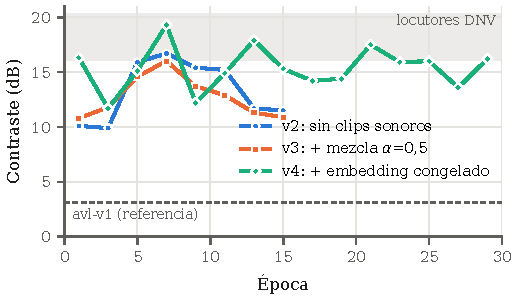
\includegraphics[width=\columnwidth]{figuras/fig_epocas.pdf}
\caption{Contraste sonora/sorda por época (una semilla). La franja gris es el rango de los locutores humanos del DNV; la línea discontinua, avl-v1.}
\label{fig:epocas}
\end{figure}

\subsection{Comparación de candidatos}
La Tabla~\ref{tab:resultados} resume los puntos de control evaluados con tres semillas.
\begin{itemize}
\item \textbf{Variantes de v4}: todas mantienen la calidad (PESQ 3,97--4,12 frente a 4,00 de avl-v1) y una inteligibilidad comparable (WER 4,4--8,1\,\% frente a 5,7\,\%).
\item \textbf{Similitud con Gina}: en v4 sube con las épocas, de 0,901 en la 5 a 0,930--0,935 a partir de la 15, y se acerca al techo de avl-v1 (0,949). La similitud con la locutora del DNV se mantiene en 0,37--0,41: Gina no se convierte en la otra voz.
\item \textbf{Prosodia}: v4 conserva la variación de F0 (4,3--5,2~st). v2 en la época 7 logra un contraste alto, pero con una entonación plana (2,84~st), por debajo del umbral fijado.
\end{itemize}

\begin{table*}[t]
\centering
\caption{Resultados por punto de control (media de 3 semillas; $\pm$ desviación típica del contraste)}
\label{tab:resultados}
\begin{tabular}{@{}llccccc@{}}
\toprule
Sistema & Época & Contraste $\Delta$ (dB) $\uparrow$ & Sim. Gina $\uparrow$ & PESQ$^{*}$ $\uparrow$ & WER (\%) $\downarrow$ & Var. F0 (st) \\
\midrule
Gina, servidor (referencia) & -- & 2,7 & 1,000 & 3,83 & 7,5 & 3,42 \\
avl-v1 & 29 & 3,1 & 0,949 & 4,00 & 5,7 & 4,81 \\
\midrule
\multirow{2}{*}{v2: filtrado} & 7 & 16,2 $\pm$ 1,2 & 0,909 & 3,94 & 6,3 & 2,84 \\
 & 11 & 13,2 $\pm$ 1,9 & 0,923 & 4,00 & 6,3 & 4,26 \\
\midrule
v3: + mezcla $\alpha{=}0{,}5$ & 7 & 14,8 $\pm$ 1,5 & 0,904 & 4,07 & 3,8 & 3,39 \\
\midrule
\multirow{9}{*}{v4: + \textit{embedding} congelado} & 5 & 16,2 $\pm$ 1,4 & 0,901 & 4,00 & 5,1 & 3,88 \\
 & 13 & 17,9 $\pm$ 0,6 & 0,922 & 4,02 & 8,1 & 5,21 \\
 & 15 & 15,5 $\pm$ 0,7 & 0,928 & 4,00 & 6,9 & 4,25 \\
 & 19 & 13,9 $\pm$ 0,5 & 0,934 & 4,12 & 7,5 & 4,43 \\
 & 21 & 14,7 $\pm$ 2,6 & 0,920 & 3,97 & 4,4 & 4,51 \\
 & 23 & 14,3 $\pm$ 2,4 & 0,935 & 4,08 & 6,3 & 5,06 \\
 & \textbf{25} & \textbf{16,5 $\pm$ 1,1} & \textbf{0,930} & \textbf{4,06} & \textbf{5,7} & \textbf{4,71} \\
 & 27 & 10,4 $\pm$ 2,8 & 0,932 & 4,04 & 5,7 & 4,33 \\
 & 29 & 14,9 $\pm$ 2,0 & 0,934 & 3,99 & 5,1 & 5,07 \\
\midrule
DNV, mujer / hombre (humanos) & -- & 16,1 / 20,3 & -- & -- & -- & -- \\
\bottomrule
\end{tabular}
\vspace{2pt}

{\footnotesize $^{*}$PESQ estimado sin referencia (TorchAudio-Squim). La fila de referencia usa una sola realización generada por el servidor.}
\end{table*}

\subsection{Análisis por clase de sibilante}
La Fig.~\ref{fig:clases} desglosa la caída por clase.
\begin{itemize}
\item \textbf{Gina original y avl-v1}: tratan /\fz/, /\fdz/ y /\fZ/,/\fdZ/ como sordas (caídas de $-29$ a $-35$\dB, iguales a las de las sordas de control).
\item \textbf{avl-v4 en la época 25}: recupera la barra de sonoridad en las tres clases: $-16{,}6$\dB{} en /\fz/, $-20{,}0$ en /\fdz/ y $-23{,}5$ en /\fZ/,/\fdZ/, valores muy próximos a los de la locutora del DNV ($-12{,}3$, $-18{,}2$ y $-23{,}6$).
\item \textbf{Sordas}: siguen siendo sordas ($-35{,}7$\dB). El modelo, por tanto, no sonoriza en exceso: restituye la oposición.
\end{itemize}

\begin{figure}[t]
\centering
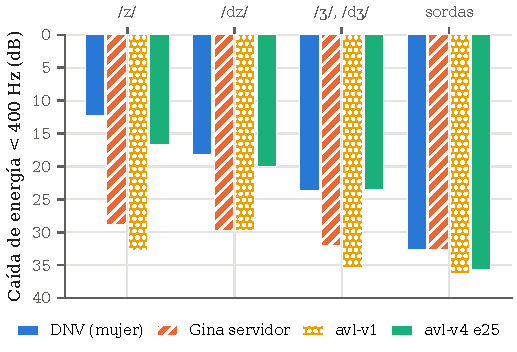
\includegraphics[width=\columnwidth]{figuras/fig_clases.pdf}
\caption{Caída de energía por debajo de 400~Hz en la zona de fricción, por clase de sibilante (barras más cortas = más sonoridad). avl-v4 e25 promedia tres semillas.}
\label{fig:clases}
\end{figure}

\subsection{Selección del modelo}
Con los criterios de la Sección~\ref{sec:eval}, varios puntos de control de v4 son aceptables. Diferencias de 1--2\dB{} entre ellos están dentro del ruido entre semillas, de modo que la elección es un compromiso entre las distintas medidas:
\begin{itemize}
\item la \textbf{época 13} ofrece el mayor contraste y el más estable (17,9$\pm$0,6\dB), pero el WER más alto;
\item la \textbf{época 25} combina un contraste de 16,5\dB, dentro del rango humano, con una similitud de 0,930, la mejor PESQ de su grupo, WER igual al de avl-v1 y una prosodia variada.
\end{itemize}
Se adopta la época 25 como modelo recomendado. La época 27 ilustra el riesgo de seleccionar con una sola semilla: con la semilla inicial daba 13,6\dB, pero con tres semillas su media cae a 10,4\dB.

% ==========================================================================
\section{Discusión y limitaciones}
% ==========================================================================

\textbf{Por qué funciona la congelación.} En v3 el \textit{embedding} mezclado es un punto de partida, pero no una restricción. La pérdida de reconstrucción sobre los clips de Gina, que siguen sonando a Gina, empuja $\mathbf{e}_7$ de vuelta hacia su posición original, y con él vuelve el ensordecimiento. Al congelarlo (v4), la única forma de reducir esa pérdida es adaptar el codificador y el decodificador. Estos se comparten con los locutores del DNV, que siempre sonorizan. Así el timbre se aprende ``alrededor'' de un punto del espacio de \textit{embeddings} que ya codifica la sonoridad. El filtrado previo de los clips (v2) es imprescindible: sin él, el decodificador recibiría ejemplos explícitos de Gina con /\fz/ realizada como [\fs].

\textbf{Limitaciones.}
\begin{enumerate}
\item No se ha completado una evaluación perceptiva formal con oyentes. Las dos pruebas habituales serían:
\begin{itemize}
\item \emph{MOS} (\textit{Mean Opinion Score}): la puntuación media subjetiva de calidad de voz que dan los oyentes, normalmente en una escala de 1 a 5;
\item \emph{ABX}: una prueba de discriminación perceptiva en la que el oyente escucha dos señales, A y B, y debe decidir a cuál de ellas se parece una tercera, X.
\end{itemize}
Se ha preparado una prueba a ciegas con las siete versiones principales, pero sus resultados no se recogen aquí.
\item El conjunto de prueba es pequeño, con 26 sibilantes en cinco oraciones. Por eso las diferencias entre puntos de control de v4 no son significativas.
\item La métrica de caída es heurística. Aunque separa con claridad las voces humanas del DNV de las voces apitxadas, no se ha validado contra juicios de oyentes.
\item Las medidas de calidad y similitud son estimaciones automáticas. Además, el reconocedor está sesgado hacia el catalán central, lo que añade ruido al WER.
\item Los datos de Gina son sintéticos, generados por el propio modelo. El techo de naturalidad lo marca, pues, la voz original.
\item Todas las medidas se han hecho con el vocoder alVoCat. La versión de producción usa WaveNeXt, y habría que comprobar que la mejora se mantiene con él.
\end{enumerate}

% ==========================================================================
\section{Conclusiones y trabajo futuro}
% ==========================================================================

El \textit{apitxat} de la voz Gina de Matxa no se corregía cambiando la fonemización ni con un ajuste fino convencional sobre datos normativos. La sonoridad de las sibilantes estaba ligada al \textit{embedding} de la locutora. La receta propuesta tiene tres pasos:
\begin{enumerate}
\item eliminar los ejemplos de la locutora que contienen sibilantes sonoras;
\item inicializar su \textit{embedding} como una mezcla al 50\,\% con un locutor normativo;
\item congelarlo durante el ajuste fino.
\end{enumerate}
Con ella, el contraste sonora/sorda pasa de unos 3\dB{} a 16,5\dB, comparable al de los locutores humanos del DNV, sin pérdidas apreciables de timbre, calidad, inteligibilidad ni prosodia.

Como trabajo futuro se plantean cuatro líneas:
\begin{itemize}
\item una prueba perceptiva con hablantes valencianos;
\item ampliar el conjunto de oraciones de prueba;
\item desplegar el modelo con el vocoder WaveNeXt del servidor de producción;
\item aplicar la técnica a otros rasgos dialectales ligados al locutor, como el vocalismo átono, y explorar la mezcla parcial por dimensiones del \textit{embedding} en lugar de la interpolación global.
\end{itemize}

\section*{Disponibilidad del código y los datos}
El código del ajuste fino, el fonemizador AVL, la métrica de caída, los scripts de evaluación, las oraciones de prueba y todas las medidas que dan lugar a las tablas y figuras están disponibles con licencia GPL-3.0 en \url{https://github.com/pexposit/apitxat-matxa}. No se distribuyen los datos del DNV, propiedad de la AVL, cuyo uso requiere su permiso previo. Tampoco se distribuyen los modelos ajustados, porque las voces de origen están restringidas a uso no comercial y de investigación.

\section*{Agradecimientos}
A Ismael Sanz, por el despliegue de las voces en el servidor de síntesis del DeepLab de la Universitat Jaume I. Al Projecte Aina y al Barcelona Supercomputing Center, por publicar Matxa y alVoCat. A la Acadèmia Valenciana de la Llengua, por el \textit{Diccionari normatiu valencià} y sus grabaciones.

\bibliographystyle{IEEEtran}
\bibliography{referencias}

\end{document}
